\documentclass[a4paper,14pt]{extarticle}

\usepackage{cmap}
\usepackage[T2A]{fontenc}
\usepackage[utf8]{inputenc}
% \UseRawInputEncoding
\usepackage[english, russian]{babel}

\usepackage{misccorr}
\usepackage{amssymb,amsfonts,amsmath,amsthm}  
\usepackage{indentfirst}
\usepackage[usenames,dvipsnames]{color} 
\usepackage[unicode,hidelinks]{hyperref}
\usepackage{makecell,multirow} 
\usepackage{ulem}
\usepackage{graphicx,wrapfig}
\graphicspath{{img/}}

\renewcommand{\labelenumii}{\theenumii)} 
\newcommand{\mean}[1]{\langle#1\rangle}

\newcommand{\numb}[1]{\,\scalebox{0.8}{\textbf{(#1)}}\,}

\DeclareMathOperator{\Div}{div}
\DeclareMathOperator{\const}{const}
%%%%%%%%%%%%%%%%%%%%%%%%%%%%%%%%%%%%%%%%%%%%%%%%%%%%%%%%%%%%%%%%%%%%%%%%%%%%%%%
%%%%%%%%%%%%%%%%%%%%%%%%%%%%%%%%%%%%%%%%%%%%%%%%%%%%%%%%%%%%%%%%%%%%%%%%%%%%%%%
\usepackage{float}
\usepackage[mode=buildnew]{standalone}
\usepackage[outline]{contour}
\usepackage{tocloft}
\renewcommand{\cftsecleader}{\cftdotfill{\cftdotsep}} % for parts
% \renewcommand{\cftchapleader}{\cftdotfill{\cftdotsep}} % for chapters
\usepackage{pgfplots,pgfplotstable,booktabs,colortbl}
\usepackage{physics}
\usepackage{mathtools}
\mathtoolsset{showonlyrefs=true}

\newcommand*\dotvec[1][1,1]{\crossproducttemp#1\relax}
\def\crossproducttemp#1,#2\relax{{\qty[\vec{#1}\times\vec{#2}\,]}}

\newcommand*\prodvec[1][1,1]{\crossproducttempa#1\relax}
\def\crossproducttempa#1,#2\relax{{\qty[{#1}\times{#2}\,]}}
% \usepackage{showframe}
\usepackage[]{geometry}
\geometry{
  left=2.5cm,
  right=1.5cm,
  top=2cm,
  bottom=2cm,
  bindingoffset=0cm,
  headheight=17pt
}
\linespread{1.5} 
% \linespread{0.9} 
\setlength{\parindent}{1.25cm}
\frenchspacing 
\usepackage{setspace,pythonhighlight}

\begin{document}

\begin{titlepage}
\begin{spacing}{1.5}


  \begin{center}
    {\fontsize{ 12pt }{ 12pt } \selectfont \bf 
    МИНИСТЕРСТВО НАУКИ И ВЫСШЕГО ОБРАЗОВАНИЯ \\[-10pt] 
    РОССИЙСКОЙ ФЕДЕРАЦИИ}\\
    \vspace{12pt}
    \begin{spacing}{1}
      {\bf  Федеральное государственное автономное \\
      образовательное учреждение высшего образования \\
      <<Национальный исследовательский Нижегородский \\ 
      государственный университет им. Н.И. Лобачевского>>
      }
    \end{spacing}
    \vspace{24pt}
    \begin{spacing}{1}
      Радиофизический факультет\\
      Кафедра общей физики\\
      \vspace{20pt}
      Направление <<радиофизика>>\\
      \vspace{20pt}
      % ОТЧЕТ ПО $\ldots$ ПРАКТИКЕ
      ОТЧЕТ ПО ПРОИЗВОДСТВЕННОЙ ПРАКТИКЕ\\
      (ПРЕДДИПЛОМНАЯ ПРАКТИКА)
      % Курсовая работа\\
      % \vspace{10pt}
      \textbf{\textsc{\Large
      % Пеленгация грозовой активности\\ \, и изучение динамики грозы  
      }}
    \end{spacing}
    \vspace{100pt}
    \begin{equation}
      \begin{aligned}
        &\text{Руководитель практики:}\quad &\text{Мареев Е.\,А.}\\
        &\text{Студент 3-го курса бакалавриата:}\quad &\text{Сарафанов Ф.\,Г.}
      \end{aligned}
    \end{equation}
  \end{center}
  \vfill
  \begin{center}
    {Нижний Новгород, 2019}
  \end{center}
\end{spacing}
\end{titlepage}

\tableofcontents
\newpage

\section*{Введение}
\addcontentsline{toc}{section}{Введение}

Важнейшим вопросом физики атмосферного электричества является зарождение и развитие грозы. Первым шагом к её рождению является разделение зарядов и формирование грозового облака.

\vspace{-1em}
\paragraph{Современное представление о грозе.} Из натурных измерений известно, что разделение зарядов происходит в следующих условиях: \numb{1} высоты между изотермами  0 $\text{C}^\circ$ и -40 $\text{C}^\circ$, \numb{2} в присутствии переохлажденной воды в жидкой фазе, \numb{3} при наличии восходящих конвективных потоков, переносящих гидрометеоры в область переохлажденной воды \cite{charge2}.

Гидрометеоры, достигая переохлажденных областей, инициируют кристаллизацию, при этом у льдинок происходит разделение заряда\footnotemark\hspace{0.02em}: на больших высотах они заряжены преимущественно положительно, на меньших (изотерма -10 $\text{C}^\circ$) -- отрицательно \cite{charge}.
\footnotetext{Наибольшую роль в разделении заряда играют безиндукционные механизмы: зарядка соударяющихся льдинок и снежной крупы в присутствии мелких водяных капель} 
Кроме этого, появляется еще более низкая (изотерма 0 $\text{C}^\circ$) и сравнительно малая положительная область со стороны Земли. При этом в облаке проводимость меньше, чем в окружающей атмосфере (где $\sigma$ экспоненциально растёт с высотой), и внутри облака не происходит постоянной нейтрализации заряда. 

Таким образом, по современным представлениям, грозовое облако имеет не
дипольную (двухслойную), а трёхслойную структуру, что хорошо подтверждается измерениями \cite{th1}.

Процесс грозовой электризации приводит к достижению пробойного потенциала и инициации разрядов. Дальнейшее развитие заряда описывается стримерно-лидерной теорией электрического пробоя.

Общее рассмотрение грозовых явлений не как локальных явлений, а глобально обусловленных электродинамикой всей Земной атмосферы ведётся в рамках теории глобальной электрической цепи (ГЭЦ). Принято считать, что грозовые облака поддерживают квазистационарное распределение токов в атмосфере: ток течёт вверх в областях грозы и вниз в областях хорошей погоды, а поверхность Земли и ионосфера замыкают цепь \cite{gec}. 
\vspace{-1em}
\paragraph{Актуальность.} Исследование гроз и их параметризация для 
развития численных моделей и количественного сопоставления реальной грозе требуют проведения большого количества натурных экспериментов для уточнения характера развития грозы, временной динамики разрядов, 
характерных временных и пространственных масштабов в зависимости от внешних условий. Имея большие массивы данных, возможно создание параметризаций атмосферы, учитывающих не только термогидродинамические явления, но и электродинамические, как один из основных факторов погодных изменений.
\vspace{-1em}
\paragraph{Цели работы.} В данной работе будут изучены результаты натурного эксперимента -- записи единичной грозы в средней полосе России, осуществлён разбор записанных данных грозы, их  статистический анализ и  классификация молниевых разрядов.





% \section{Динамика разряда и грозопеленгация}
% 
% \subsection{Конвекция и перенос заряда в атмосфере}

% Как было установлено в ряде работ [1, 3, 4], пограничный слой атмосферы характеризуется наличием аэроэлектрических структур (рис. 1), проявляющихся в короткопериодных (с периодами от единиц до нескольких сотен секунд) пульсациях электрического поля. Формируясь в результате захвата турбулентными конвективными ячейками положительных и отрицательных заряженных частиц, аэроэлектрические структуры перемещаются в потоке воздуха. Конвективный перенос заряда аэроэлектрическими структурами служит важнейшим механизмом формирования электрического тока в глобальной цепи. В связи с этим представляют большой интерес механизмы генерации и время существования электрических структур, связанные, в частности, с влиянием аэрозолей на время релаксации электрического заряда в конвективных ячейках [3, 6]. Особое значение имеет разработка и реализация методов мониторинга конвекции с помощью разнесенных наблюдений вертикального квазистатического аэроэлектрического поля. Такой мониторинг может послужить мощным средством оперативной диагностики ППС и верификации новых представлений о геофизической турбулентности.

\newpage
\section{Натурный эксперимент}

Аппаратура, размещенная на территории пункта Городец, позволяла вести наблюдения электрического и магнитного полей в грозовых условиях. Флюксметр регистрировал медленные изменения электрического поля ($<$10 Гц). Для наблюдения сигналов ближних гроз в СДВ диапазоне (500-10000 Гц) использовалась трехкомпонентная приемная система (две компоненты горизонтального магнитного поля и одна компонента вертикального электрического поля). 


Сигналы с приемной системы поступали на АЦП и после дискретизации записывались на накопитель. Установка работала в непрерывном режиме, генерируя поток данных около $700$ Мб/ч. Чтобы увеличить время непрерывной записи до заполнения накопителя, запись производилась в пороговом режиме. 

На предшествующих измерениях была определена средняя амплитуда электрического поля регистрируемого молниевого разряда при грозе на расстоянии 100 км от датчиков. При амплитуде ниже пороговой АЦП работал на частоте дискретизации $f_\text{slow}=20$ Гц (медленный режим); при превышении амплитудой порога оцифровка велась на на частоте $f_\text{fast}=20$ кГц (быстрый режим). Спустя час быстрого режима, если отсутствовали импульсы выше порогового, АЦП переходил в медленный режим.


\subsection{Фильтрация и сглаживание данных с флюксметра}

Для упрощения работы алгоритма пик-детектора статическое поле 
было отфильтровано от помехи 50 герц и её гармоник с помощью цифрового фильтра Баттерворта 3-го порядка. 

Отфильтрованные данные сглаживаются оконным фильтром Савицкого-Голея , который при правильном подборе ширины окна позволяет сгладить сигнал, не теряя данных о пиках \cite{sav} (простое сглаживание сплайнами, например, при резких скачках данных может значительно их исказить). Сглаживание необходимо для меньшей зашумленности производной.

Обработанные и необработанные данные показаны на рисунке \ref{fig:peak-detection}, стр. \pageref{fig:peak-detection}.


\subsection{Программная реализация пик-детектора}

Для обработки полученных в ходе измерений данных было необходимо
решить ряд программных задач. Выделение из массива данных
временных интервалов, пригодных к временной и пространственной локализации молнии, осуществлялось с помощью цифрового пик-детектора.

На массиве данных методом скользящего окна \cite{stat} рассчитывается дискретная производная по времени от медленного электрического поля, усредняемая на ширине окна $\Delta T$. 

При превышении производной порога фиксируется момент времени $t_1$. Начиная с этого момента и до следующего превышения порога (в отрицательную сторону), выделяется интервал данных. В нем содержится атмосферик\footnotemark, и чтобы заведомо не потерять данных о разряде, интервал расширяется влево и вправо на $t_\text{padding}$. 
\footnotetext{В физике атмосферы атмосфериком (а иногда короче -- сфериком) называют поле, распространяющееся от разряда молнии.}

Ширина окна, уширение интервала и порог производной являются параметрами пик-детектора, и их можно  подобрать различными способами: \textbf{(1)} исходя из априорной информации (длительность молниевого разряда, сила тока разряда, уровень шума, известные помехи), \textbf{(2)} или непосредственно по обрабатываемым данным, разметив вручную на временной шкале примерные точки разряда и методом последовательных итераций подбирая параметры, чтобы они наилучшим образом реализовали поиск пиков.

\begin{figure}[h!]
  \centering
  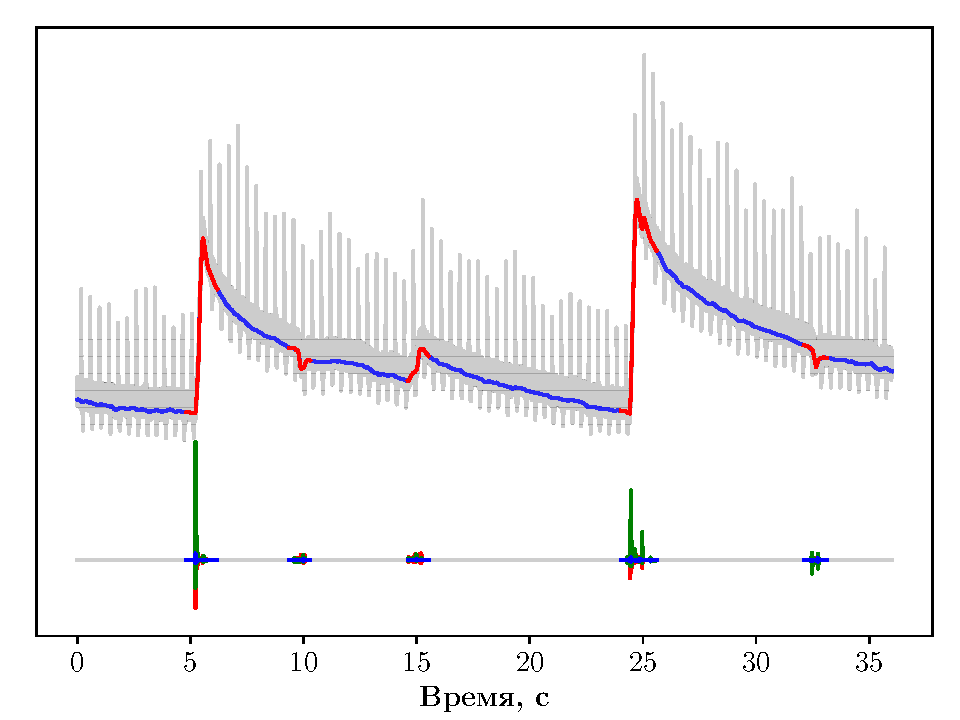
\includegraphics[width=\textwidth,trim={0cm 0cm 0cm 0cm},clip]{fig/peak-detection.pdf}
  \caption{Фиксация цифровым пик-детектором квазистатических
  изменений электрического поля}
  \label{fig:peak-detection}
\end{figure}

Для данной работы был реализован второй вариант. На рис. \ref{fig:peak-detection} можно видеть работу пик-детектора: найденные пики показаны на кривой статического поля красным цветом.


\subsection{Определение атмосфериков}

На каждом пике определяется амплитуда скачка статического поля, а по знаку скачка разряды классифицируются как <<облако-земля>> и <<земля-облако>>. Разряды с малой амплитудой скачка статического поля и большой амплитудой быстрого поля вне зависимости от знака скачка можно с трактовать как внутриоблачные разряды: именно они могут не изменить статического поля (заряд остался в облаке, перераспределившись).

Классификация разрядов затрудняется тем, что одинаковую регистрируемую картину могут иметь как далекие сильные разряды (статическое поле от них почти не меняется) так и близкие не очень сильные внутриоблачные разряды.
Без привлечения дополнительных данных (например, регистрация грома) их разделение достаточно условно, и требует дополнительных исследований. Один из способов разделения -- по временной структуре (или спектру) атмосферика.

В временном интервале атмосферика (см. рис. \ref{ris:field}б) ищется глобальный экстремум магнитного поля. Экстремум является первым разрядом молнии, в точке экстремума определяются составляющие магнитного поля, по которым можно определить направление на разряд.

\begin{figure}[h]
\begin{minipage}[h]{0.49\linewidth}
\centering
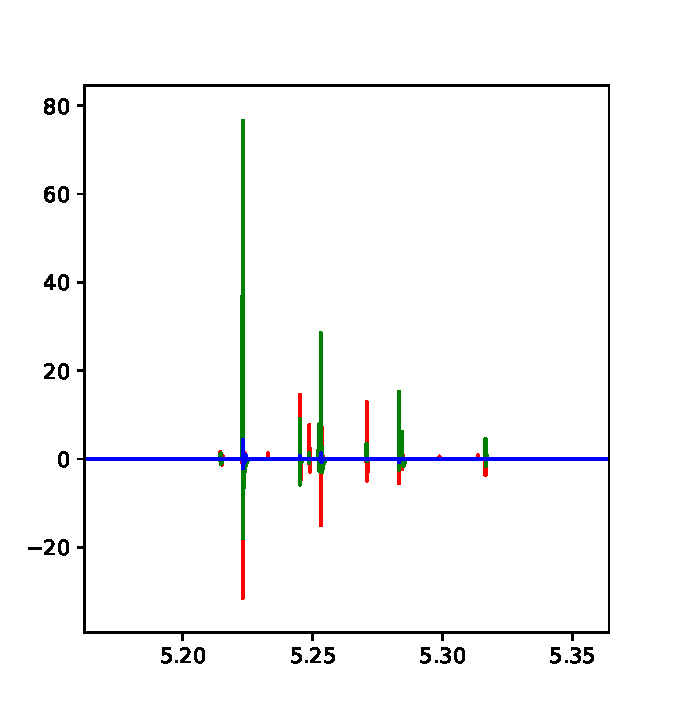
\includegraphics[height=1.1\linewidth]{fig/multiple}\\
\hspace{1em}а) Многокомпонентный разряд
\end{minipage}
\hfill
\begin{minipage}[h]{0.49\linewidth}
\center{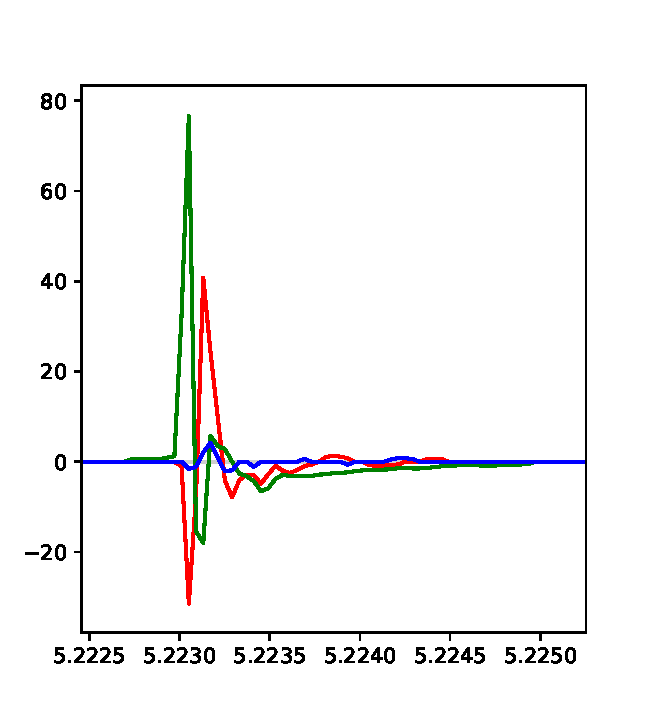
\includegraphics[height=1.1\linewidth]{fig/one} \\ б) Атмосферик разряда}
\end{minipage}
\vspace{0.7em}
\caption{Поля разряда молнии}
\label{ris:field}
\end{figure}

Существуют т.н. многокомпонентные разряды (см. рис. \ref{ris:field}a): в одном канале молнии с интервалом 20-60 мкс происходит несколько последовательных разрядов. Такие последовательности также анализируются с помощью программы (см. приложение 1), и регистрируется количество компонент. 

\begin{figure}[H]
  \centering
  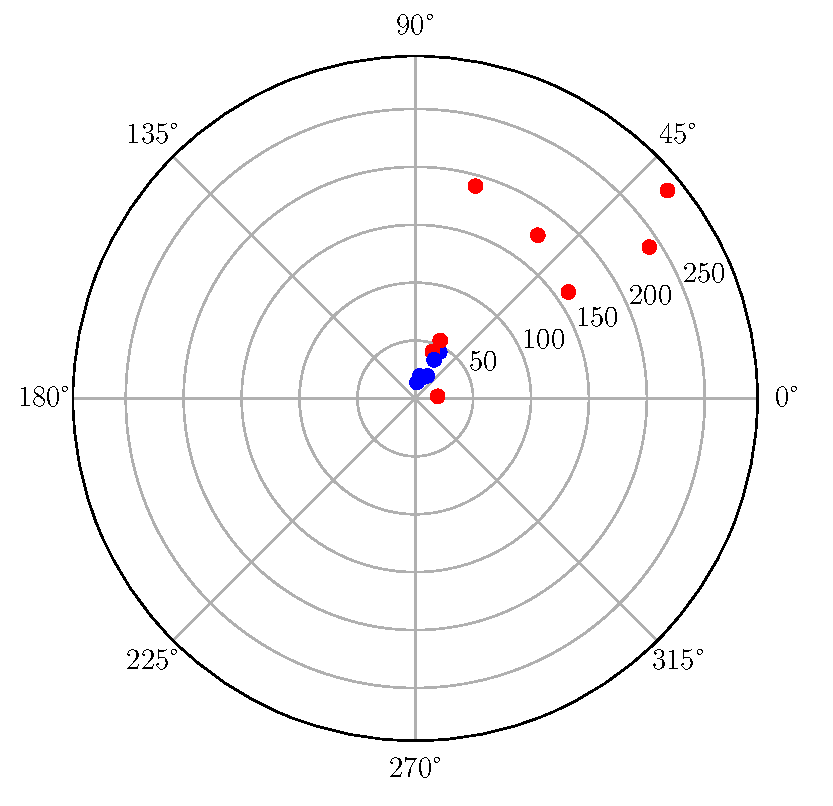
\includegraphics[scale=0.9]{fig/str}
  \caption{Радарная карта ударов молнии за 90 секунд}
  \label{fig:strikes_map}
\end{figure}

Таким образом, в итоге программной обработки имеются набор данных о разрядах: для каждого разряда получены время разряда, амплитуда скачка статического поля, направление на разряд, амплитуда магнитного поля первой компоненты разряда, количество компонент разряда, тип разряда (облако-земля, земля-облако, облако-облако). 

По полученным данным можно осуществлять грозопеленгацию (см. рис. \ref{fig:strikes_map}) и исследовать характер отдельных стадий грозы, интегральные характеристики и т.п.

\newpage
\section{Динамика квазистатического поля грозы}
\subsection{Положение грозового облака}

Для анализа записанного квазистатического поля, которое наблюдается только в ближней зоне грозы, необходимо знать расстояние для грозы. При сильном сносе
грозового облака относительно наблюдателя нельзя отличить медленное изменение поля, обеспеченное удалением источника, от изменения поля в результате коллективных процессов зарядки.

\begin{figure}[H]
  \centering
  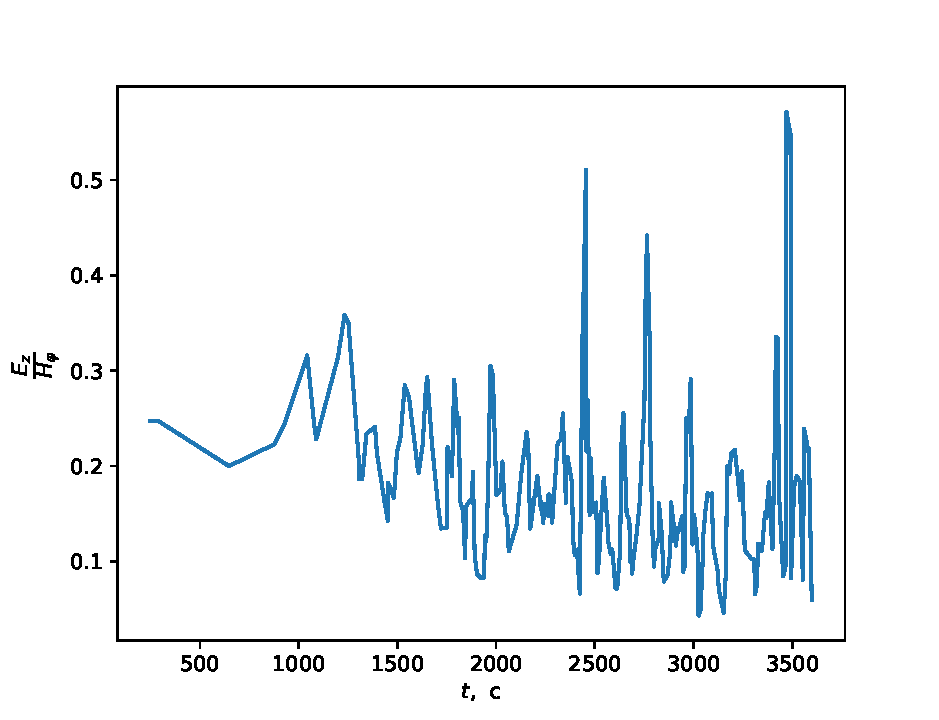
\includegraphics[scale=1]{fig/frac.pdf}
  \caption{Отношение амплитуд полей разрядов}
  \label{fig:frac}
\end{figure}

Чтобы обосновать пренебрежение зависимостью положения облака для конкретного измерения, воспользуемся $E-H$ методом. В приближении вертикального дипольного излучателя, а также считая Землю идеальным проводником, можно найти поля (в СИ) \cite{rp}:
\begin{equation}
  E_z = \frac{k^{2}}{2 \pi \varepsilon_{0}}\left[1-\frac{1}{j k R}+\frac{1}{(j k R)^{2}}\right] \frac{e^{j k R}}{R} P(j \omega) e^{-j \omega t}
\end{equation}
\begin{equation}
  H_{\varphi}=-\frac{k^{2} c}{2 \pi}\left[1-\frac{1}{j k R}\right] \frac{e^{j k R}}{R} P(j \omega) e^{-j \omega t},
\end{equation}
где $R$ -- расстояние до излучателя, $P(j\omega)$ -- дипольный момент излучателя.

В ближней зоне отношение амплитуд будет функцией от расстояния. Для данной грозы зависимость приведена на рис. \ref{fig:frac}.

Действительно, можно видеть, что хотя и отдельные разряды происходят на разном расстоянии, с течением времени средняя удаленность разряда изменяется меньше, чем на характерный размер грозы (который определяется максимальным и минимальным расстоянием до разряда).


\subsection{Зависимость квазистатического поля от времени}
Как упоминалось во введении, процесс зарядки грозового облака обычно обусловлен безындукционным механизмом зарядки, в котором разделение электрического заряда происходит за счет различия физико-химических свойств соударяющихся частиц, а соударение происходит за счёт энергии среды. При этом рост поля облака происходит линейно, что часто наблюдается при анализе грозорадарных данных \cite{charge}.

Реже наблюдается, что при формировании грозового облака и развитии грозы поле растёт с экспоненциальной составляющей во времени. В записи, исследуемой в данной работе, именно этот случай (см. рис. \ref{fig:charge}). Покажем, что это может быть следствием индукционной зарядки.

  % (энергетически - энергия разделения заряда возникает из-за диссипации турбулентной энергии). 
\begin{figure}[H]
  \centering
  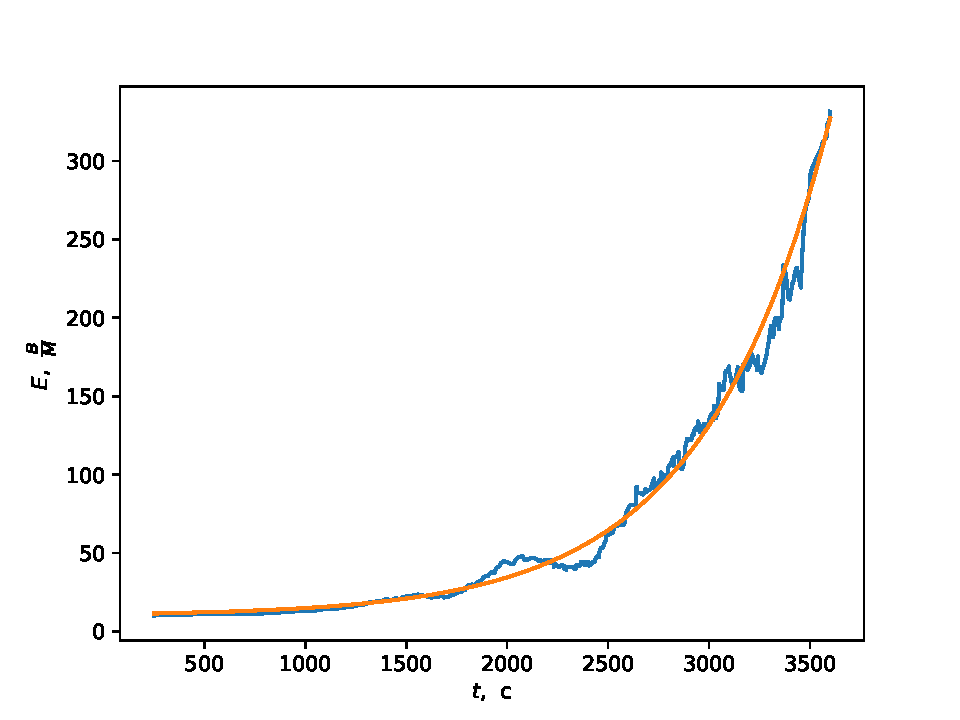
\includegraphics[]{fig/charge.pdf}  
  \caption{Экспериментально измеренное поле грозы}
  \label{fig:charge}
\end{figure}

Теория индукционной зарядки строится в предположении, что все частицы можно отнести к большим и малым, с характерными размерами $r$ и $E$. В грозовом облаке это  снежная крупа радиусом 0.4-4 мм и льдинки радиусом 5-100 мкм.% [27, 101, 125]
 
Как показано в работе \cite{dem}, при индукционном механизме разделения зарядов ток зарядки определяется выражением (формула получается совместным решением уравнения баланса токов, динамики частиц с учетом вязкости и турбулентных течений в плоской модели)
\begin{equation}
  J_{z}=\frac{3 \xi r^{2} n N}{\left(N+\gamma \frac{r^{2}}{R^{2}} n\right)} E \cdot\left|U_{z}\right|
\end{equation}
где $U_z$ -- это относительная скорость больших и малых частиц, $r,R$ -- радиусы частиц, $n,N$ -- концентрации частиц, $\xi$ и $\gamma$ -- безразмерные параметры ($\xi$ характеризует поляризацию, а $\gamma$ -- отношение радиусов частиц)


Усредняя ток зарядки и считая, что $\mean{|U_1|}=\sqrt{\mean{U_1^2}}$), можно получить выражение для тока зарядки, возникающего за счет турбулентных флуктуаций (энергетически -- за счет диссипации турбулентной энергии):
\begin{equation}
  \mean{J_z} = \beta E_0,
\end{equation}
где $\beta$ -- коэффициент, определяемый рядом микропараметров грозового облака, имеющий размерность проводимости.

Действительно, при определенных значениях микропараметров может быть так, что $\beta>\sigma$ (где $\sigma$ -- проводимость среды), и в таком случае можно наблюдать экспоненциальный рост электрического поля. Натурные эксперименты показывают, что 
с ростом размеров облака относительный вклад индукционного механизма растет, и для характерных больших грозовых ячеек может достигать порядка $25\%$.


\newpage
\section*{Заключение}
\addcontentsline{toc}{section}{Заключение}

В работе изучены некоторые характеристики отдельной грозы. Проведена работа по обработке бинарных данных с установки, написана программа для разбора данных и грозопеленгации, при этом создан алгоритм цифрового пик-детектирования по первой производной величины. 

\vspace{-1em}
\paragraph{Преимущества созданной программы.} Существующие проприетарные грозорадары не позволяют анализировать самостоятельно данные о грозе, выдавая только рассчитанную по записанным данным радарную информацию. Созданная программа позволит собрать массив данных по грозам, отличающийся от предыдущих выделением не только радарной информации о разряде, но и отрезков данных, которые могут предоставлять интерес для обучения нейросетевых погодных моделей с учетом электродинамических явлений (существующие модели обычно учитывают их только как параметры, в т.н. индексных методах).

\vspace{-1em}
\paragraph{Результаты обработки данных.} По результатам обработки часовой записи грозы в Городце исследованы так же некоторые макро-характеристики: положение грозы и характер зарядки грозы. Сделан вывод о наличии индукционного механизма зарядки.

\vspace{-1em}
\paragraph{Перспективное развитие работы.}  В экспериментальной части планируется полный цикл создания зонд-флюксметра для уточнения распределения поля в нижних слоях атмосферы: проектирование схемы, создание прототипа и испытания. В теоретической части планируется \numb{1} развить подход использования $E-H$ метода с переходом к более сложной (и реалистичной) геометрии задачи и учётом конечной проводимости подстилающей поверхности.
\numb{2}На основе уточненных данных о распределении статического поля также возможно дальнейшее исследование процессов  зарядки грозового облака. 









\newpage
\addcontentsline{toc}{section}{Список литературы}
\begin{thebibliography}{99}
\bibitem{charge2} Дементьева С.О. О динамике разделения зарядов в грозовых облаках -- Нижний Новгород, Россия, 2015. -- 20 с.

\bibitem{charge} Mansell E.R. Charge structure and lightning sensitivity in a simulated multicell thunderstorm  -- Journal of Geophysical Research -- 2005. -- Т. 110 -- № D12 -- С.D12101.


\bibitem{th1} Kuettner J. The electrical and meteorological conditions inside thunderclouds -- Journal of Meteorology -- 1950. -- Т. 7 -- № 5 -- С.322–332.

\bibitem{gec} Cлюняев Н.Н.  Теоретическое исследование структуры и динамики глобальной электрической цепи : автореферат диссертации на соискание учёной степени кандидата физико-математических наук -- Нижний Новгород, Россия, 2016 -- 27 с.

\bibitem{dem} Дементьева С.О. Процессы коллективной зарядки в нижней атмосфере и их описание в численных мезомасштабных моделях : автореферат диссертации на соискание учёной степени кандидата физико-математических наук -- Нижний Новгород, Россия, 2019 -- 20 с.



\bibitem{rp} Бару Н.В., Кононов И.И., Соломоник М.Е. Радиопеленгаторы-дальномеры ближних гроз -- М.:Гидрометеоиздат, 1976 - 144 с.

\bibitem{sav} Ляхов А. А., Шкуркин В. В. Применение фильтров Савицкого-Голея для обработки вольтамперных характеристик зондов Ленгмюра -- Вестник ОмГУ, 2012. №4 (66). 

% \bibitem{land} Ландау Л.Д., Лифшиц Е.М. Теоретическая физика: т.5, Статистическая физика. - М.: Физматлит, 2005. - 616 с.

\bibitem{stat} Грешилов А. А., Стакун В. А., Стакун А. А. Математические методы построения прогнозов. -- М.: Радио и связь, 1997. -- 112 с.
\end{thebibliography}

\newpage
\section*{Приложение 1. Код пик-детектора}
\addcontentsline{toc}{section}{Приложение 1. Код пик-детектора}

Программа написана на языке Python версии 3.7.0, с библиотеками NumPy 1.15.2 и SciPy 1.2.1. Время обработки  -- 2-10 секунд (в зависимости от производительности ПК) работы кода на 36 секунд входных данных. 
\vspace{1em}
\begin{spacing}{0.9}
\inputpython{py/code_print_en.py}{1}{192}
\end{spacing}

\end{document}